\documentclass[border=10pt]{standalone}
\usepackage{tikz}
\usetikzlibrary{patterns}
\begin{document}
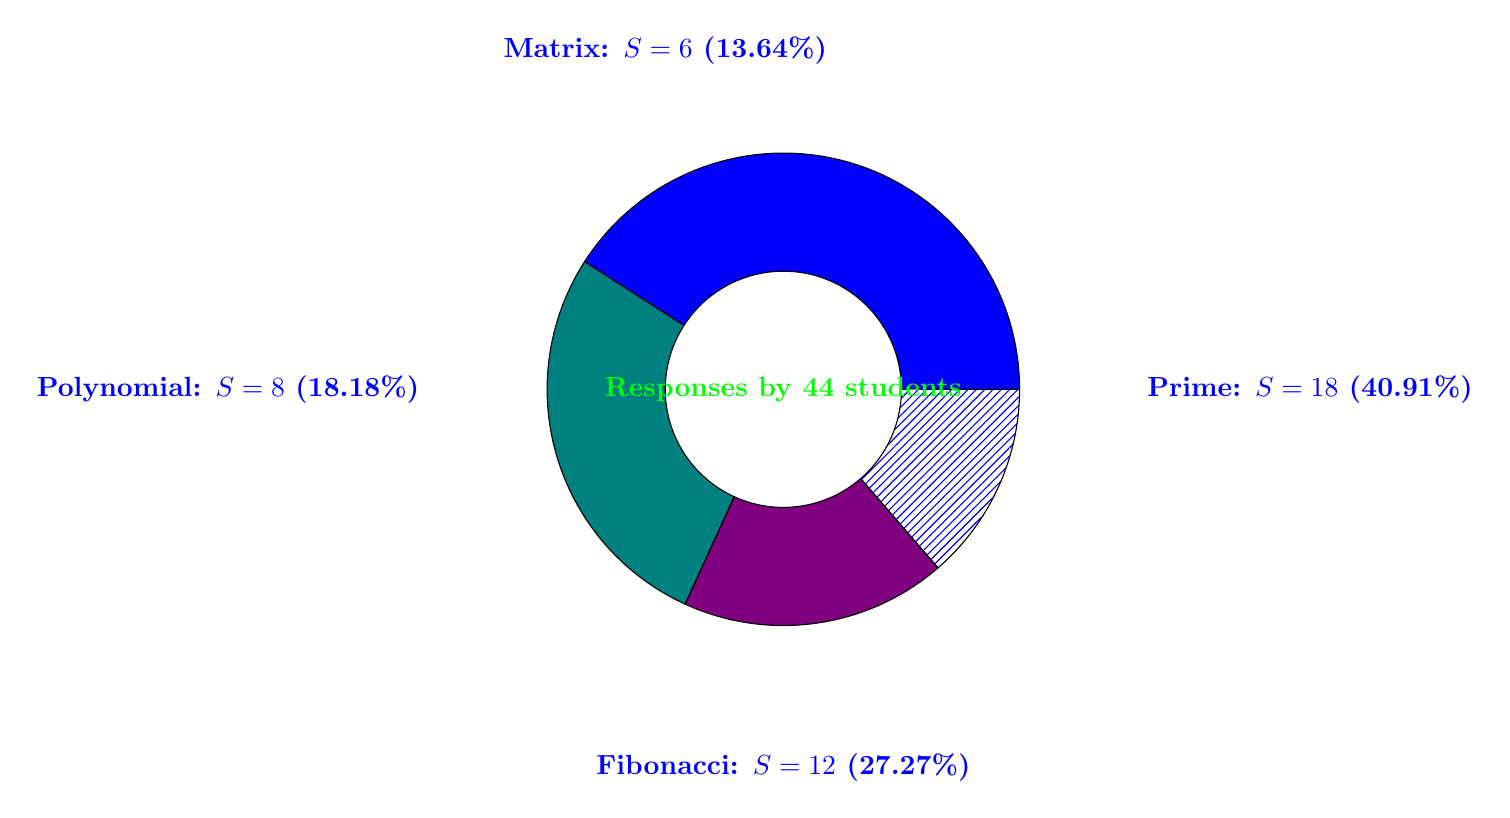
\begin{tikzpicture}
% Define colors and radii
\def\innerradius{1.5cm}
\def\outerradius{3cm}

% Prime segment (Blue)
\draw[fill=blue] (0:\outerradius) arc (0:147.276:\outerradius) -- (147.276:\innerradius) arc (147.276:0:\innerradius) -- cycle;
% Fibonacci segment (Teal)
\draw[fill=teal] (147.276:\outerradius) arc (147.276:245.448:\outerradius) -- (245.448:\innerradius) arc (245.448:147.276:\innerradius) -- cycle;
% Polynomial segment (Purple)
\draw[fill=violet] (245.448:\outerradius) arc (245.448:310.896:\outerradius) -- (310.896:\innerradius) arc (310.896:245.448:\innerradius) -- cycle;
% Matrix segment (Orange with pattern)
\draw[fill=orange, pattern=north east lines, pattern color=blue] (310.896:\outerradius) arc (310.896:360:\outerradius) -- (0:\innerradius) arc (0:-49.104:\innerradius) -- cycle;

% Center text
\node[green, font=\bfseries] at (0,0) {Responses by 44 students};

% Labels
\node[blue, font=\bfseries] at (4.5,0) [anchor=west] {Prime: $S = 18$ (40.91\%)};
\node[blue, font=\bfseries] at (0,-4.5) [anchor=north] {Fibonacci: $S = 12$ (27.27\%)};
\node[blue, font=\bfseries] at (-4.5,0) [anchor=east] {Polynomial: $S = 8$ (18.18\%)};
\node[blue, font=\bfseries] at (-1.5,4) [anchor=south] {Matrix: $S = 6$ (13.64\%)};
\end{tikzpicture}
\end{document}